\section{A Chain of Trust for the TEM}\label{concepts:trust_chain}

Section \ref{concepts:guarantees} shows that trusted execution requires that a
secret be established between Yu and Mii's computer that Yu trusts. This
section describes a chain of trust that allows Yu to assert that a public key
corresponds to a private key that can only be found inside a computer Yu
trusts. The chain of trust was derived by removing the unnecessary parts from
the chain of trust used for platform attestation in the TPM \cite{tcpa2007}.

\begin{figure}[bhp]
	\center{
		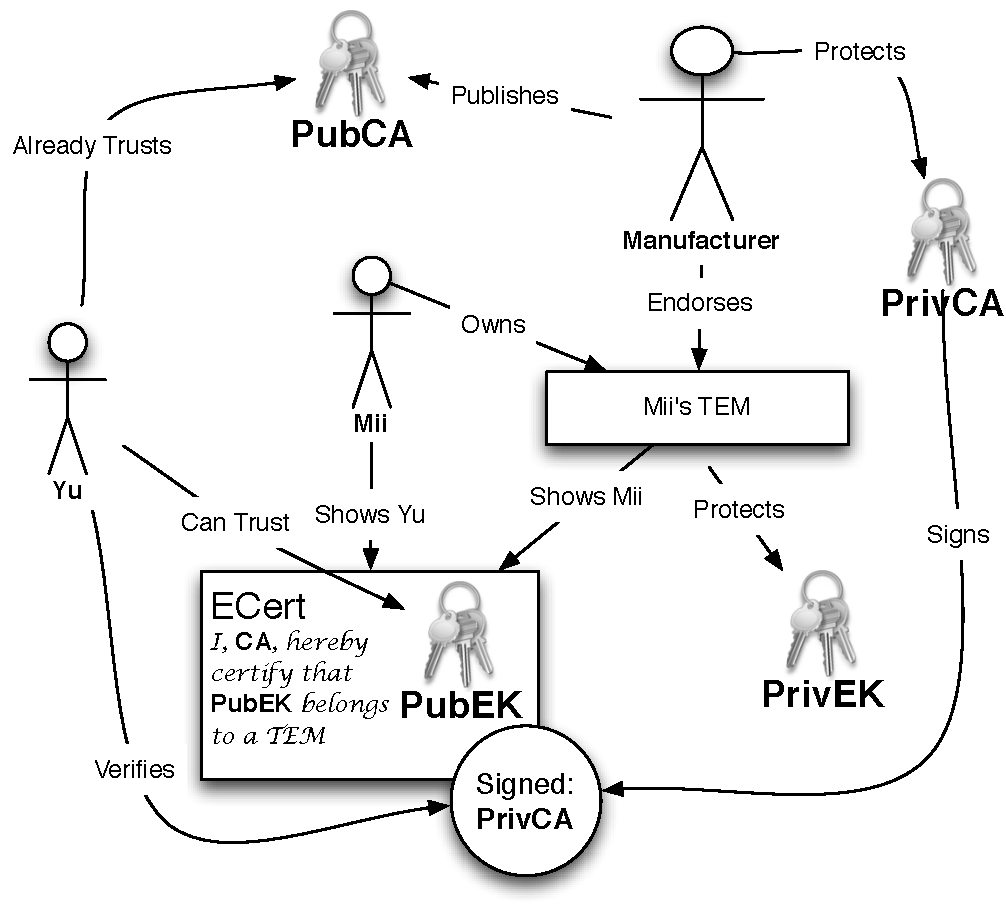
\includegraphics{omnifigs/trust_chain}
	}
	\caption{The Chain of Trust Used by Yu to Trust the TEM }
	\label{fig:trust_chain}
\end{figure}

The public and private keys in this section can use any public-key encryption
system, such as RSA \cite{rivest1978mod} or ECC \cite{koblitz1987ecc}. Figure
\ref{fig:trust_chain} illustrates the chain of trust.

The root of trust is a hardware manufacturer (such as Infineon or Atmel), which
acts as a Certificate Authority in a public key infrastructure as defined in
\cite{housley2002ixp}. The manufacturer has an asymmetric key named the
Certificate Authority key. This key consists of protects the private key
(PrivCA), while the public key (PubCA) is assumed to be well known.

At TEM manufacturing time, an asymmetric key, called an Endorsement Key,
is generated for each TEM. The Private Endorsement Key (PrivEK) is securely
embedded into the TEM. Then the manufacturer's private key (PrivCA) is used to
sign an Endorsement Certificate (ECert) containing the TEM's Public
Endorsement Key (PubEK), and stating that the Endorsement Key has been embedded
in a hardware device that provides the security guarantees required by a TEM.

The TEM's Public Endorsement Key can be used to encrypt a secret generated
by Yu, which becomes the shared secret between Yu and Mii's TEM needed to
satisfy the requirement in \ref{concepts:guarantees}. Once Mii presents Yu with
his TEM's Endorsement Certificate, she is assured that any secrets encrypted
with PubEK can only be decrypted by Mii's TEM, as it is the only computer that
knows PrivEK. This method allows for secret information to flow securely from
Yu to Mii's TEM. If there is a need for secret information to flow the other
way, Yu can send Mii's TEM a symmetric\footnote{Building symmetric encryption
features into the TEM requires careful consideration, because most countries
regulate the use of symmetric encryption algorithms.} or
asymmetric encryption key, which is protected as described above, and allows for secure
communication of secrets in both directions.

As stated towards the beginning of this section, the chain of trust is rooted
at the hardware manufacturer who emits the Endorsement Certificate. Readers
troubled by the need to trust big manufacturers should note that they have
probably entrusted their information to small stores and credit unions, as well
as to people working for various institutions.

\subsection{Anonymizing the TEM}\label{concepts:anonymous_trust}
The chain of trust above has a potential issue: the proof that a TEM can be
trusted requires the Public Endorsement Key. Since a TEM has exactly one PubEK,
the PubEK can be used to identify and track the TEM, and thus its owner. This
may be unacceptable in some circumstances, as it leaks information about the
users' identity, just like the Intel Processor Serial Number (PSN)
\cite{gengler1999isi}, which has generated great public uproar. Fortunately,
the chain of trust described above can be amended in a way that makes the TEM
untraceable.

The threat to anonymity stems from the fact that a TEM has a single Public
Endorsement Key, which acts as a shared secret between the TEM and Yu, so Yu
sees the same PubEK every time she interacts with Mii's TEM. This can be
improved by adding an extra layer of keys, as follows.

In the modified design, when Mii needs to interact with Yu, he instructs his
TEM to create a new asymmetric User Key, which is handled similarly to the
Endorsement Key. The Private User Key (PrivUK) is never disclosed by the TEM,
and the Public User Key (PubUK) is included in a User Certificate (UCert)
signed by the TEM's Private Endorsement Key (PrivEK). The User Certificate
states that the User Key was generated by the TEM, and the appropriate security
guarantees hold.

Mii sends the User Certificate, together with the Endorsement Certificate, to a
trusted server maintained by the TEM's manufacturer. The server verifies the
two certificates to make sure that the Public User Key was indeed generated by
a TEM emitted by the manufacturer, then the server gives Mii a User Endorsement
Certificate (UECert) signed by the manufacturer's private CA key (PrivCA), and
stating that the User Key provides all the security guarantees of a TEM User Key.

At the end of the process Mii can use the User Endorsement certificate to prove
that the User Key can be trusted just as much as an Endorsement Key. However,
UECert does not contain any information identifying the particular TEM used to
generate the User Key. So this mechanism makes the TEM untraceable.

The process described in this section does not require any special-purpose
mechanism in the TEM. The steps above can be implemented in the TEM as programs
on top of the architecture presented in chapter \ref{arch}, which was designed
without regard to this section. Therefore, the information here does not
pertain to the TEM's design. Rather, it is included as to pacify any anonymity
concerns that a reader may have.
